\section{Introduction}
In the context of single-agent path finding A* \cite{hart68} is regarded as 
the gold standard search algorithm.
It is complete, optimal and optimally efficient which makes it very attractive 
to researchers in the area.
Many studies exist which have attempted to improve on the performance of A* in pathfinding. 
The majority focus in one of two directions: reducing the search space through hierarchical 
decomposition and identifying better heuristics to guide search. 
In the case of hierarchical decomposition, techniques such as
HPA*~\cite{botea04} and PRA*~\cite{sturtevant05} seek to construct and explore
a much reduced approximate state space.
This makes them very fast. 
They also require no significant extra-memory when compared to A*.
However, they have the disadvantage that solutions are not guaranteed to be optimal.
Meanwhile, in case of the improved heuristics, it has been frequently shown
that obtaining better informed results than than the popular
Manhattan heuristic usually incurs significant memory overhead 
\cite{sturtevant09,goldberg05,Cazenave:06,bjornsson06}.
Furthermore it is well known that even heuristics which differ from perfect information 
by at most a (small) additive constant, can still exhibit poor performance on a range of 
problems such as AI planning and path finding \cite{helmert08,pohl77}.
%Our simple example shown in Figure \ref{fig-emptymap}, which we discuss later,
%shows a similar behaviour in path finding.
\par
%When compared to a standard pathfinding method, such as A* with a Manhattan heuristic,
%all techniques outlined so far involve some kind of performance trade-off.
%They are typically faster than A* but, at the same time, require significant
%extra memory or provide no optimality guarantees.
In this paper we explore a new speedup technique that aims to reduce the size of the search 
space while preserving optimality.
Our work focuses on eliminating symmetric path segments from 4-connected grid maps,
which allow straight but not diagonal movement. 
Although less popular than the 8-connected variant, this domain appears regularly in the 
literature  \cite{yap02,wang08,pochter09} and is often found in the pathfinding systems of modern video games.
Some recent examples include Square Enix's \emph{Heroes of Mana} (released for the Nintendo DS),
Astraware's \emph{My Little Tank} (iPhone) and Atari's \emph{Dragon Ball Z: Legacy of Goku} 
(Gameboy Advance). 
\par
Consider as a motivating example the simple map in Figure \ref{fig-overview}.
%, which
%requires finding a path from one room on the map to another.
Such topographies, with rooms and corridors, appear often in video games 
(e.g., dungeon areas in roleplaying games
can be described in such terms, albeit on a larger scale).
Running A* on a standard grid can be surprisingly inefficient in such instances.
%For many locations on the map, including all tiles in rooms A, C and E, the Manhattan heuristic
%is almost perfect, as it differs from the true distance by almost two.
In Figure~\ref{fig-overview}, many tiles have \emph{f-values} smaller than the goal's,
and A* must expand them.
Many of the explored paths are symmetric in the sense that they can be obtained from each other
by re-ordering the moves.

\begin{figure}[tb]
       \begin{center}
                       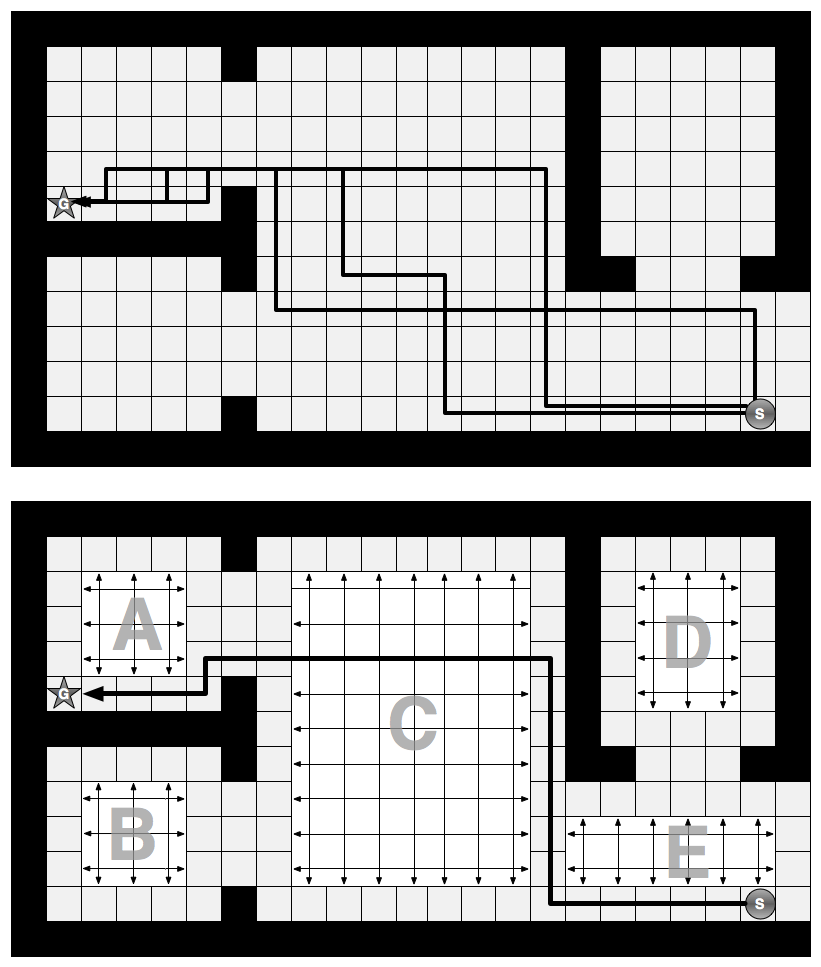
\includegraphics[scale=0.30, trim = 10mm 10mm 10mm 0mm]{diagrams/overview.png}
       \end{center}
	\vspace{-3pt}
       \caption{(Top) A highly symmetric pathfinding instance that is simple to humans but difficult 
				for a computer.
				Many solutions exist; we highlight three. 
				(Bottom) The same map with our symmetry elimination method applied. We decompose the map
				into a set of obstacle-free rooms from which we prune all nodes except those on the perimeter.
				We replace them with a small set of macro edges that connect the perimeter nodes directly.} 
       \label{fig-overview}
\end{figure}

To solve the problem more efficiently we will automatically discover obstacle-free rectangular rooms and 
observe that while there are many ways to optimally traverse across a room there is always a solution 
involving only nodes from the perimeter.
This observation forms the basis for our symmetry elimination technique: we prune all nodes from the interior
but not the perimeter of an empty room and, to preserve optimality,
replace them with a series of \emph{macro edges} that allow
moving directly from one side of an empty room to the other. 
In the process we eliminate almost all equivalent path segments when crossing a room,
significantly reducing the number of locations that must be explored.
Cases when the start (or the goal) location belongs to the interior of an empty rectangle are handled by
temporarily re-inserting these nodes back into the map.
\par
Our method is easy to understand and implement.
It produces grid maps that are often much smaller than the original grid map
(and never larger), have the same branching factor and preserve the same completeness and optimality 
guaranteeing characteristics.
Further, since our method is focused on eliminating symmetries in the search space, it is orthogonal to existing 
search techniques, including both hierarchical and low level pathfinding systems as well as memory-based heuristics.
We demonstrate its effectiveness by undertaking an empirical analysis on a wide range of maps, 
including a well known set from the popular roleplaying game \emph{Baldur's Gate II}. 
On our test data the average number of A* node expansions is reduced by up to a
factor of three.
We also report a corresponding search time speedup of up to four times, depending on the 
topography of the map being used.
% \par
% The rest of the paper is structured as follows.
% Next we overview related work. Then we provide a formal description of our 
% symmetry elimination technique.
% Following that we discuss how to decompose the traversable part of a grid map into a partition 
% of empty areas.
% Finally we present our experiments and results just before our conclusions and future work ideas.

%%%%
%We will exploit this property in order to identify and eliminate a large number of nodes from the
%associated graph.

%In addition to appearing frequently, 4-connected grid maps are also highly symmetric; i.e.
%there are usually many optimal length paths between any given pair of points. 
%Symmetry is unwated in search problems <something like Toby's intro>
%We exploit this property 

%Our work is inspired by hierarchical pathfinding systems such as HPA* \cite{botea04} but also shares
%commonalities with symmetry elimination techniques that are used used to speed up search in areas 
%such as constraint programming \cite{walsh}.
